\documentclass[11pt,letterpaper]{article}

% include figures
\usepackage{graphicx}
% get nice colors
\usepackage{xcolor}

% change default font to Palatino (looks nicer!)
\usepackage[latin1]{inputenc}
\usepackage{mathpazo}
\usepackage[T1]{fontenc}
% load some useful math symbols/fonts
\usepackage{latexsym,amsfonts,amsmath,amssymb,wasysym}

% comfort package to easily set margins
\usepackage[top=1in, bottom=1in, left=1in, right=1in]{geometry}

% spacing after a paragraph
\setlength{\parskip}{.15cm}
% indentation at the top of a new paragraph
\setlength{\parindent}{0.0cm}


\begin{document}

\begin{center}
\Large
Ay190 -- Worksheet 5\\
Daniel DeFelippis\\
Date: \today
\end{center}

%%
%%
%% I worked with Scott Barenfeld
%%
%% All python code can be found in the ws4 directory in my repository
%%
%%

\section{Curve Fitting}
In this worksheet, we seek to find a relationship between the 
mass of a supermassive black hole at the center of a galaxy 
and the the stellar velocity dispersion of that galaxy using 
data from Greene and Ho. 

\subsection*{a}

After downloading the data and the AstroPy package, we make a
log-log scatterplot of the data - that is, $\log_{10}M_{BH}$ vs 
$\log_{10} \sigma_{*}$ - shown in figure~\ref{fig:5a}. There is clearly
a positive relationship between the two quantities, which we will
quantify in parts b and c.

\begin{figure}[bth]
\centering
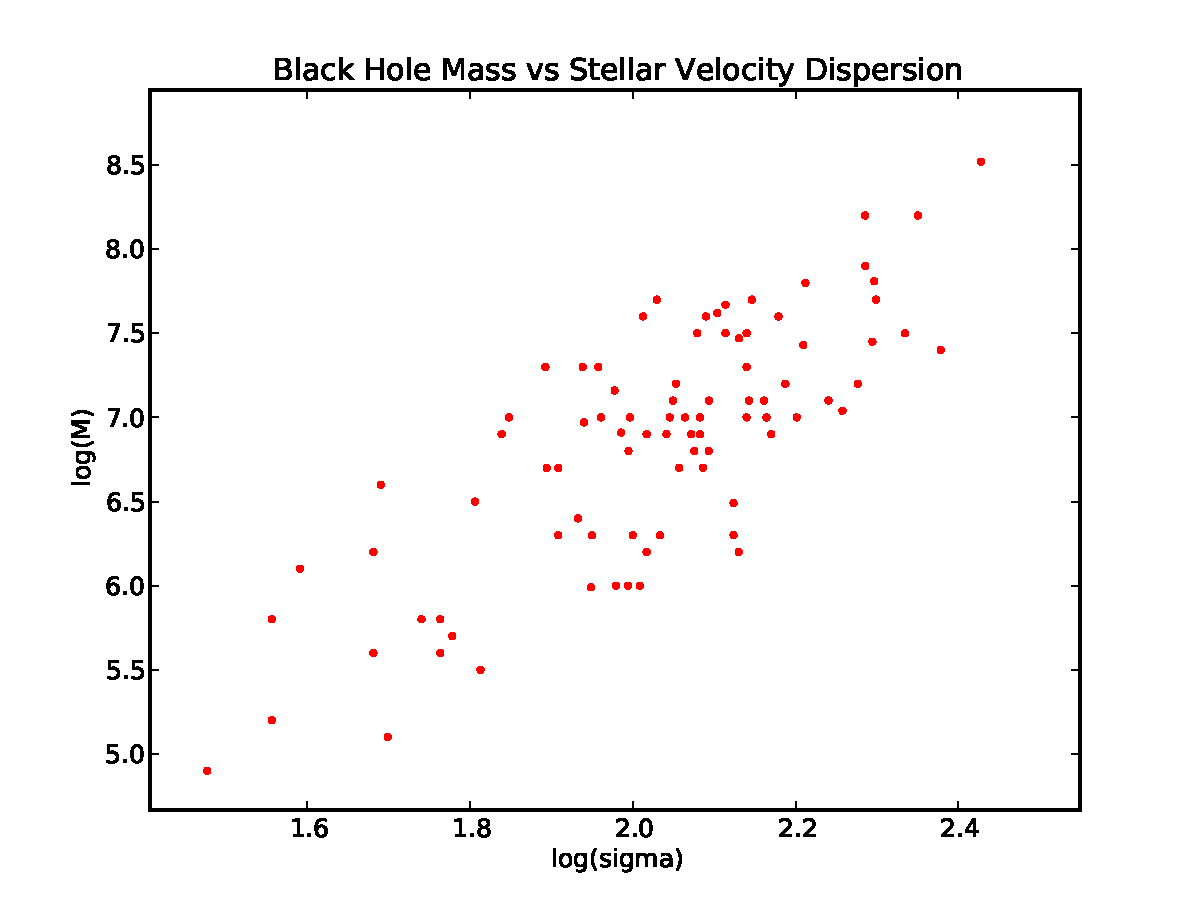
\includegraphics[width=0.75\textwidth]{ws5-a.pdf}
\caption{Log of black hole mass vs Log of stellar velocity dispersion}
\label{fig:5a}
\end{figure}


\subsection*{b}

We use formulae given in the notes to calculate 
regression line fit parameters. If we let $ x_i = (\log_{10} \sigma_{*})_i$ 
and $ y_i = (\log_{10}M_{BH})_i$, then:
$$ S = \sum\limits_{i=1}^{N} \frac{1}{\sigma_i^2}, \hspace{5pt} \Sigma x = 
\sum\limits_{i=1}^{N} \frac{x_i}{\sigma_i^2}, \hspace{5pt} \Sigma y = 
\sum\limits_{i=1}^{N} \frac{y_i}{\sigma_i^2}, \hspace{5pt} \Sigma x^2 = 
\sum\limits_{i=1}^{N} \frac{x_i^2}{\sigma_i^2}, \hspace{5pt} \Sigma xy = 
\sum\limits_{i=1}^{N} \frac{x_i y_i}{\sigma_i^2}. $$

Then, performing the fit, we get that $y = a_1 + a_2 x$ where
$$ a_1 = \frac{\Sigma y \Sigma x - \Sigma x \Sigma xy}{S\Sigma x^2 - (\Sigma x)^2},
\hspace{8pt} 
a_2 = \frac{S \Sigma xy - \Sigma x \Sigma y}{S\Sigma x^2 - (\Sigma x)^2} $$
and the uncertainties on the $a_i$ are given by
$$ \sigma_{a_1} = \sqrt{\frac{\Sigma x^2}{S\Sigma x^2 - (\Sigma x)^2}},
\hspace{8pt}
\sigma_{a_2} = \sqrt{\frac{S}{S\Sigma x^2 - (\Sigma x)^2}}.$$
Since we are ignoring the errors right now, we take $\sigma_i = 1$, 
so $S = 88$ (there are 88 data points). Calculating these parameters gives
\begin{align*}
a_1 &= 0.931069678176 \pm 1.11588027837 \\
a_2 &= 2.92542900883 \pm 0.547497898246
\end{align*}
The data and the regression line are shown together in figure~\ref{fig:5b}. 

\begin{figure}[bth]
\centering
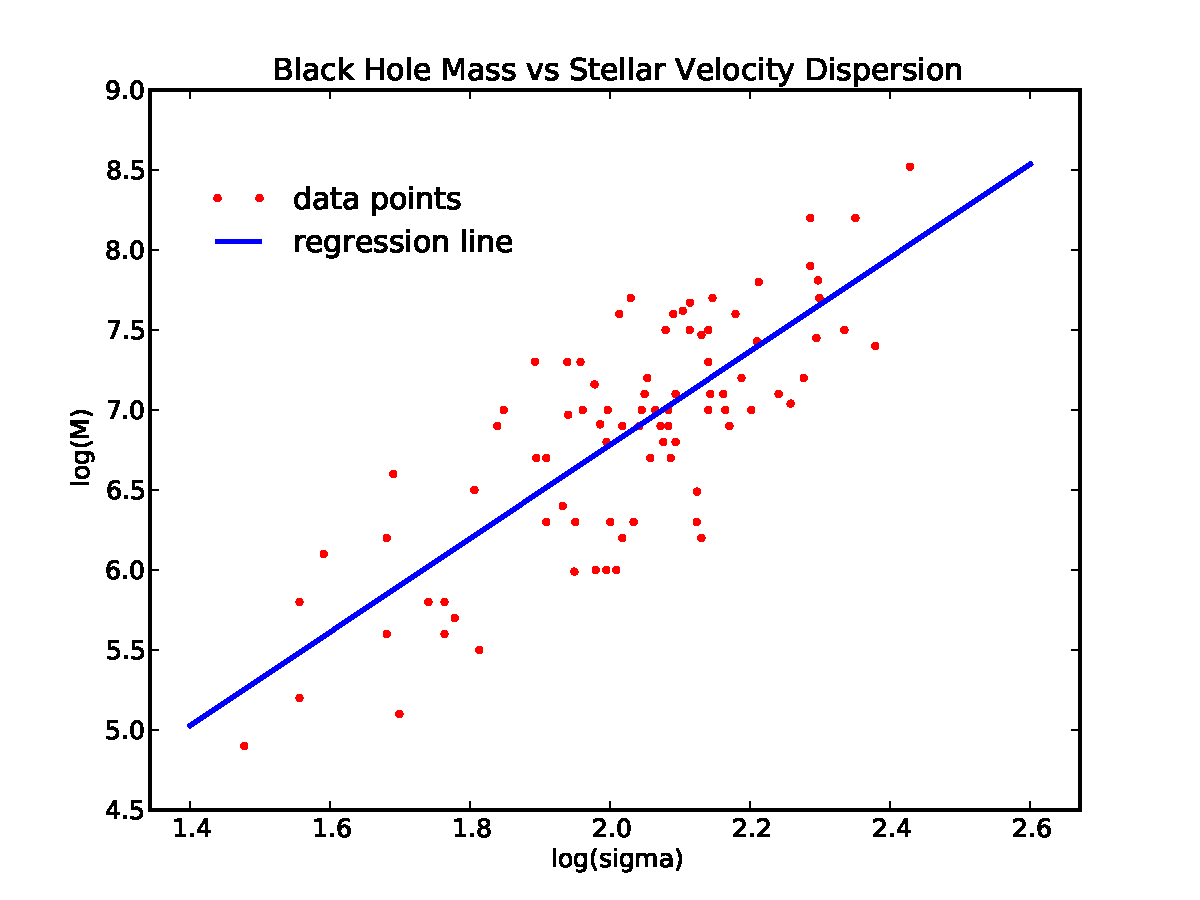
\includegraphics[width=0.75\textwidth]{ws5-b.pdf}
\caption{Log-Log data and regression line}
\label{fig:5b}
\end{figure}

We can compare our fit to the one from Greene and Ho. They fit the line
$$ \log(M_{BH} / M_{\astrosun}) = \alpha + \beta \log(\sigma_* / \sigma_0) $$ where 
$\sigma_0 = 200$ km/s, and got $\alpha = 7.85 \pm 0.04$ and $\beta = 3.69 \pm 0.13$.
Now, our $a_1$ corresponds to $\alpha - \beta \log\sigma_0$. 
The data points $log(M_{BH})_i$ are really $\log(M_{BH} / M_{\astrosun})$, so no
correction involving $M_{\astrosun}$ is needed. Also, our $a_2$ still 
corresponds to their $\beta$. 
Comparing the parameters, we see that:
\begin{align*}
a_1 &= 0.93 \pm 1.12 & \alpha - \beta \log\sigma_0 &= -0.64 \pm 0.14 \\
a_2 &= 2.93 \pm 0.55 & \beta &= 3.69 \pm 0.13
\end{align*}
which agree fairly well with each other.

\subsection*{c}

Now, including the errors, we can perform another fit. For the $\log M$ data points,
we choose to use the errors in the data file labeled "e\_logM" and for the 
$\log\sigma$ points, we choose the errors labeled "e\_sigma*". Now, we need
to transform the errors on $\sigma$ to get errors on $\log\sigma$. To do this, we
note that 
$$d(\log\sigma_*)= \frac{1}{\ln(10)} \frac{d\sigma_*}{\sigma_*},$$
so the errors on $\log\sigma_*$ are given by 
$$\frac{1}{\ln(10)} \frac{e\_sigma^*}{\sigma_*}.$$

Also, we need to combine the x and y errors, and to do that we need a value of 
$\frac{dy}{dx}$. We choose the slope $a_2$ from the previous fit as this value
for all data points, so that we can write
$$ \sigma_{i,total}^2 = (e\_\log M)_{i}^2 + \left(\frac{dy}{dx}\right)^2(e\_sigma^*)_i^2. $$
Proceding exactly as before otherwise, we calculate that 
\begin{align*}
a_1 &=  0.713709687178 \pm 0.226477686432 \\
a_2 &= 3.04393787988 \pm 0.107907788743.
\end{align*}
The graph of this fit together with the data points and their errors 
is shown in figure~\ref{fig:5c}.

\begin{figure}[bth]
\centering
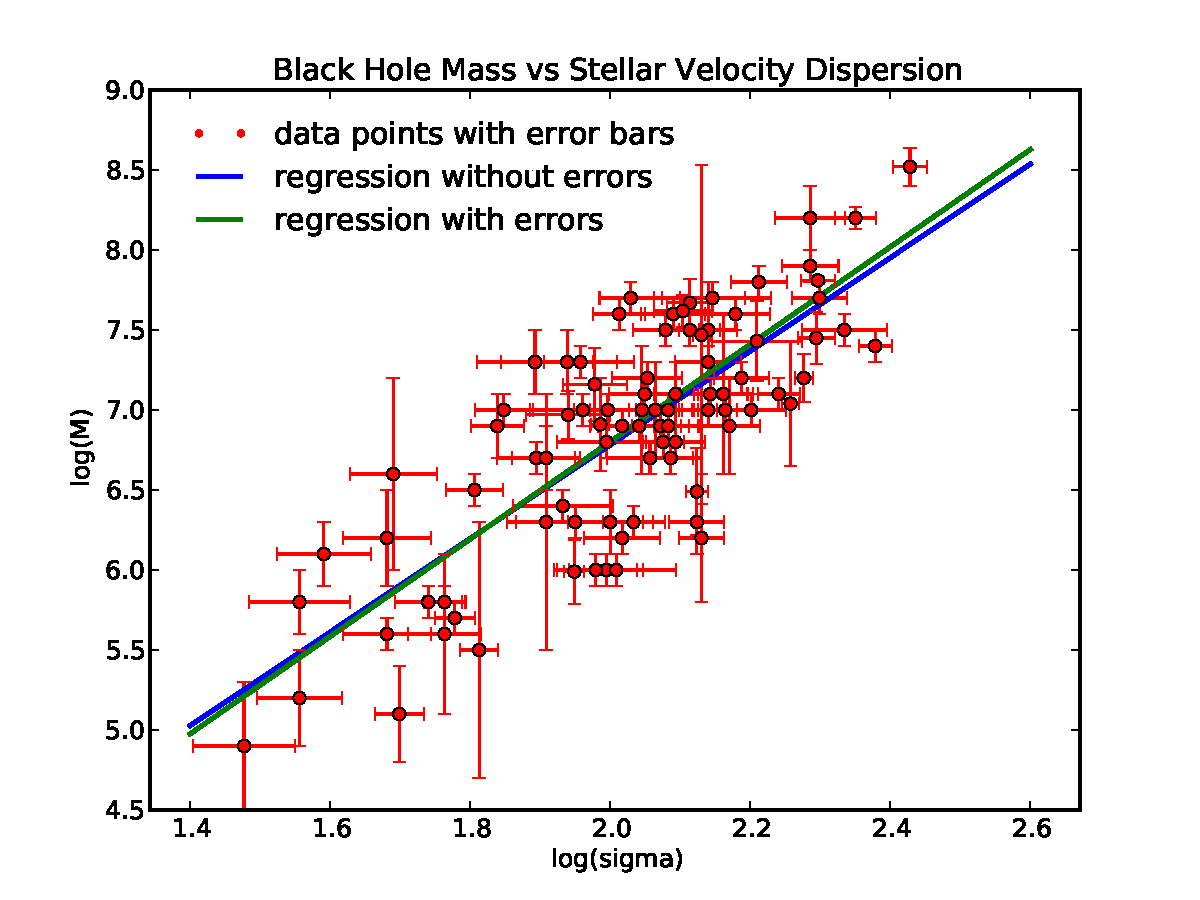
\includegraphics[width=0.75\textwidth]{ws5-c.pdf}
\caption{Log-Log data and the two regression lines}
\label{fig:5c}
\end{figure}

It is interesting to note that the uncertainties 
on both parameters went down, although now they are further from what Greene 
and Ho calculated, which suggests that there is some subtlety that I am ignoring
when I chose the errors I did.

\end{document}